\subsubsection{Prijava za praktičnu obuku}

\vspace{3mm}

\begin{itemize}

\item \textbf{Kratak opis:} Da bi kandidat započeo praktičnu obuku potrebno je da se prijavi. Pre prijave kandidat dostavlja auto školi potvrde o obavljenom lekarskom pregledu, uplatama, nakon čega bira instruktora.

\vspace{2mm}

\item \textbf{Učesnici} \newline
   - Kandidat \newline 
   - Administrativni radnik.

\item \textbf{Preduslovi:} \newline
   - Kadidat je položio teorijski ispit. \newline 
   - Kandidat je obavio lekarski pregled. 

\item \textbf{Postuslovi:} \newline
    - Kandidat se prijavio za praktičnu obuku 

\item \textbf{Osnovni tok:}  
   \begin{enumerate}
   \item Kandidat pristupa veb stranici i otvara formular za prijavu za praktičnu obuku.
   \item Kandidat popunjava formular.
   \item Kandidat klikom na dugme "Prijavi" salje prijavu.
   \item Administrativni radnik proverava ispravnost i potpunost podataka.
   \item Administrativni radnik potvrdjuje prijavu i kandidatu salje spisak slobodnih instruktora.
   \item Kandidat proverava mejl i bira instruktora.
   \item Sistem belezi prijavu kandidata i izabranog instruktora.
   \end{enumerate}

\item \textbf{Alternativni tok:}  
   \begin{itemize}
   \item A1. \textbf{Neispravnost ili nepotpunost dokumentacije:}
  Dokumentacija koju je korinik priložio je nepotpuna ili sadrži neke neispravne podatke. Slučaj upotrebe se privremeno zaustavlja dok kandidat ne kompletira potrebnu dokumentaciju ili ispravi prosleđene podatke i proces se nastavlja od koraka 1 u osnovnom toku.
  \item A2. \textbf{Kandidat nije dobio mejl:}
  Administrativni radnik nije posalo mejl o potvrdi prijave i spisak slobodnih instruktora kandidatu. proces se nastavlja od koraka 5 u osnovnom toku
   \end{itemize}

\end{itemize}  

\begin{figure}[H]
  \begin{center}
      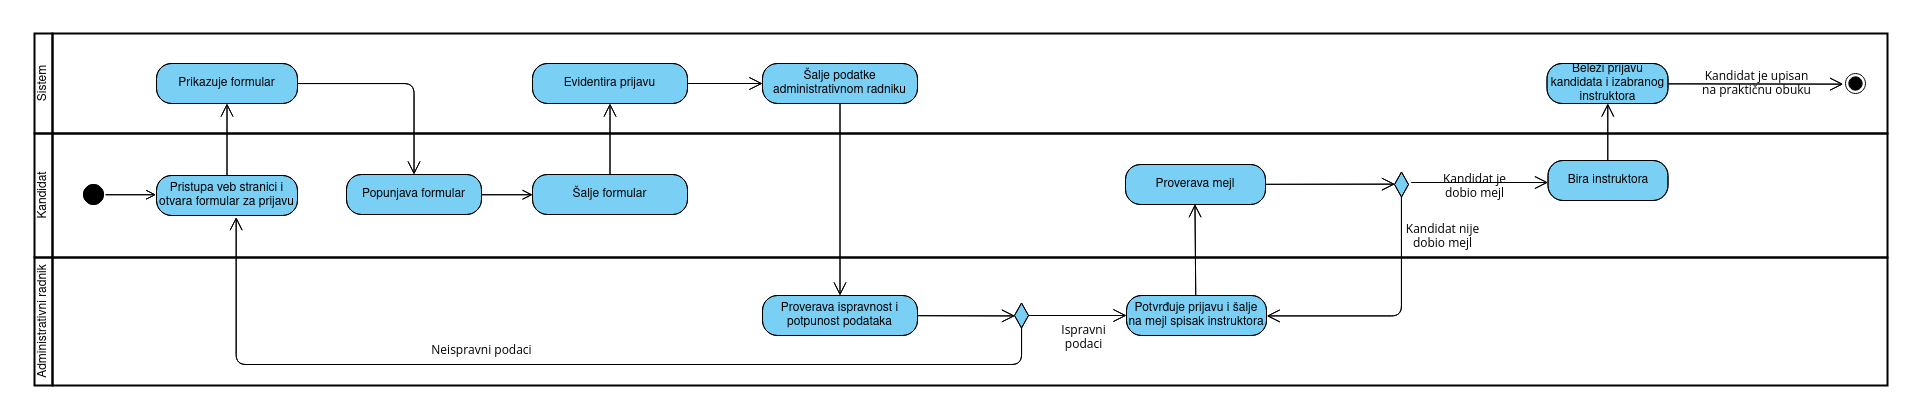
\includegraphics[width=140mm, height=70mm]{Diagrams/dijagram_aktivnosti_prijava_za_prakticnu_obuku.png}
  \end{center}
  \caption {Dijagram aktivnosti - Prijava za praktičnu obuku}
  \label{activity_prijava_za_prakticnu_obuku}

\end{figure}
